\section{Results}

\subsection{Topic Models}

The first result of performing LDA is the inferred topic models.
Because LDA is an unsupervised process there are no labels or summaries associated with the topics, only a nominal identifier.
To directly judge the semantics of a topic a human must interpret the terms and their associated frequency and extrapolate shared semantics.
Over several runs of LDA with various parameterization, different quality topics were extracted.
Table~\ref{tab:topics} displays a small selection of topics --- in this run, five hundred topics were inferred across the corpora.
The complete list of inferred topics is available online\footnote{\href{https://employability.rouly.net/web/topics}{employability.rouly.net/web/topics}}.

\begin{table}
  \centering
  \begin{tabular}{l r}
    \multicolumn{2}{c}{\small{\textbf{Topic 16}}} \\
    {\small\textit{Term}} & {\small\textit{Frequency}} \\
    \hline
    test & 0.0132 \\
    data & 0.0128 \\
    software & 0.0115 \\
    design & 0.0107
  \end{tabular}
  \begin{tabular}{l r}
    \multicolumn{2}{c}{\small{\textbf{Topic 273}}} \\
    {\small\textit{Term}} & {\small\textit{Frequency}} \\
    \hline
    market & 0.0250 \\
    product & 0.0113 \\
    strategi & 0.0107 \\
    digit & 0.0103
  \end{tabular}
  \begin{tabular}{l r}
    \multicolumn{2}{c}{\small{\textbf{Topic 418}}} \\
    {\small\textit{Term}} & {\small\textit{Frequency}} \\
    \hline
    branch & 0.0224 \\
    rental & 0.0167 \\
    enterpris & 0.0155 \\
    manageri & 0.0146
  \end{tabular}
  \begin{tabular}{l r}
    \multicolumn{2}{c}{\small{\textbf{Topic 424}}} \\
    {\small\textit{Term}} & {\small\textit{Frequency}} \\
    \hline
    care & 0.0346 \\
    nurs & 0.0179 \\
    health & 0.0168 \\
    clinic & 0.0117
  \end{tabular}
  \caption{Four inferred topics.}~\label{tab:topics}
\end{table}

\subsection{Domain Overlap}

From an LDA run with five hundred topics, ten topics were identified as ``strictly overlapping'' for certain thresholds.
Namely, $|\Omega(\rho=0.02, \theta=0.055)| = 10$.
For a set of five hundred total topics, this produces a Jaccard index of 0.02.
Table~\ref{tab:overlap} displays the ten strictly overlapping topics in $\Omega(\rho=0.02, \theta=0.055)$.
Notice that the topics in Table~\ref{tab:topics} are a subset of the topics rendered in Table~\ref{tab:overlap}.
Figure~\ref{fig:overlap} gives an additional visual reference of the complete strictly overlapping set of topics.
The closer the two bars are to equal for a given topic, the more similar that topic's distribution is within each data set.


\begin{table}
  \centering
  \begin{tabular}{l r r r r}
    & \multicolumn{4}{c}{\small{\textbf{Topic Expression}}} \\
    & \multicolumn{2}{c}{\small{\textbf{Career Data}}} & \multicolumn{2}{c}{\small{\textbf{Curricular Data}}} \\
    {\small\textit{Topic}} & {\small\textit{Count}} & {\small\textit{\%}} & {\small\textit{Count}} & {\small\textit{\%}} \\
    \hline
    16 & 9,274 & 23.43 & 568 & 9.77 \\
    273 & 8,873 & 22.42 & 583 & 10.02 \\
    274 & 2,240 & 5.66 & 1,117 & 19.21 \\
    345 & 2,676 & 6.76 & 543 & 9.34 \\
    390 & 3,130 & 7.91 & 356 & 6.12 \\
    418 & 3,069 & 7.75 & 426 & 7.32 \\
    419 & 2,590 & 6.54 & 553 & 9.51 \\
    424 & 5,561 & 14.05 & 499 & 8.58 \\
    425 & 11,807 & 29.83 & 388 & 6.67 \\
    434 & 3,793 & 9.58 & 349 & 6.00
  \end{tabular}
  \caption{Strictly overlapping topics for $\rho=0.02$ and $\theta=0.055$}~\label{tab:overlap}
\end{table}


\begin{figure}
  \centering
  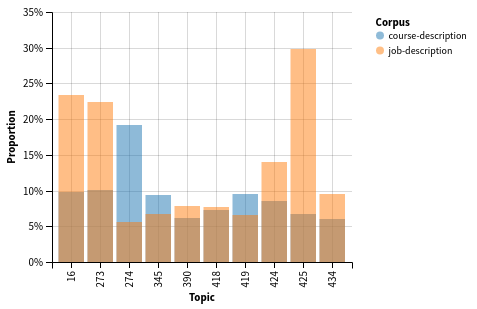
\includegraphics[width=0.5\textwidth]{figs/strict-overlap}
  \caption{Strictly overlapping topics for $\rho=0.02$ and $\theta=0.055$}~\label{fig:overlap}
\end{figure}
